\subsection{VALIDAÇÃO DE CONFIGURAÇÕES}

Devido à grade quantidade de configurações necessárias para parametrizar a geração de uma grade horária, erros de configurações por parte dos usuários são inevitáveis. Tendo isto em mente, implementou-se uma seção de cótigo no otimizador, responsável pela validação das informações providenciadas pelo usuário.

Vale ressaltar que esta validação não garante que é possível gerar uma grade horária de acordo com as configurações providas, mas ela deve evitar alguns dos erros mais comuns. As validações realizadas foram:

\begin{enumerate}
	\item Existem turnos, turmas, professores e matérias configurados;
	\item O total de aulas configurado para cada sala deve ser correto, de acordo com o número de dias da grade horária e quantidade de aulas por dia;
	\item Para cada sala, nenhum professor pode ter mais aulas agendadas do que a sala acomoda;
	\item Nenhum professor pode ter mais aulas constantes configuradas do que o seu total de aulas naquela sala;
	\item Não pode haver uma restrição e aula constante para determinado professor na mesma posição da grade horária;
	\item Cada grupo de alinhamento deve relacionar duas turmas diferentes, e referenciar o alinhamento da mesma quantidade de aulas em ambas as salas, sendo esta quantidade compatível com o total de aulas configurado para cada professor;
	\item O número de aulas esperado para cada região deve ser compatível com o total de aulas configurado para as salas englobadas na região
\end{enumerate}

Estas validações são executadas antes do início das otimizações das grades horárias, e caso haja algum erro de configuração, é exibida uma mensagem alertando o usuário, conforme a \autoref{fig:erroValidacao}, e a geração da grade horária é cancelada.

\begin{figure}[!htb]
	\centering
	\caption{Mensagem de erro de validação}
	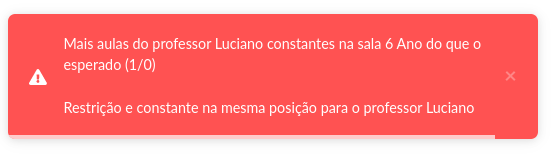
\includegraphics[width=1\textwidth]{./dados/figuras/erroValidacao}
	\fonte{Autor}
	\label{fig:erroValidacao}
\end{figure}
\pagebreak
